\documentclass[letterpaper,11pt]{article}

\usepackage{amsmath}
\usepackage{amssymb}
\usepackage[hmargin=1.25in,vmargin=1in]{geometry}
\usepackage{booktabs}
\usepackage{graphicx}
\usepackage{hyperref}
\usepackage{lmodern}
\usepackage{microtype}
\usepackage{pdflscape}
\usepackage{subcaption}

\title{Coursework 4: STAT 570}
\author{Philip Pham}
\date{\today}

\begin{document}
\maketitle

\begin{enumerate}
\item Consider the so-called Neyman-Scott problem in which
  $Y_{ij}\mid \mu_i,\sigma_2 \sim_{\mathrm{ind}}
  \mathcal{N}\left(\mu_i,\sigma^2\right), i=1,\ldots,n,j=1,2.$
  \begin{enumerate}
  \item Obtain the MLE of $\sigma^2$ and show that it is inconsistent. Why does
    this inconsistency arise in this example?

    \begin{description}
    \item[Solution:] The likelihood is
      \begin{align}
        L\left(\mu,\sigma\right)
        &= \prod_{i=1}^n \prod_{j=1}^2 \frac{1}{\sqrt{2\pi\sigma^2}}\exp\left(
          -\frac{1}{2\sigma^2}\left(Y_{ij} - \mu_i\right)^2
          \right) \nonumber\\
        &= \prod_{i=1}^n \frac{1}{2\pi\sigma^2}\exp\left(
          -\frac{1}{2\sigma^2}\left[
          \left(Y_{i1} - \mu_i\right)^2
          +\left(Y_{i2} - \mu_i\right)^2
          \right]
          \right),
          \label{eqn:p1_likelihood}
      \end{align}
      so the log-likelikehood is
      \begin{equation}
        l\left(\mu,\sigma\right) = -n\log\left(2\pi\right) -n\log\left(\sigma^2\right)
        - \frac{1}{2\sigma^2}\sum_{i=1}^n\left[
          \left(Y_{i1} - \mu_i\right)^2
          +\left(Y_{i2} - \mu_i\right)^2\right].
        \label{eqn:p1_log_likelihood}
      \end{equation}

      Taking the derivative with respect to $\sigma^2$, we have
      \begin{equation}
        \frac{\partial}{\partial\sigma^2}l\left(\mu, \sigma^2\right)
          = -\frac{n}{\sigma^2} +
          \frac{1}{2\left(\sigma^2\right)^2}\sum_{i=1}^n
          \left[
            \left(Y_{i1} - \mu_i\right)^2 +
            \left(Y_{i2} - \mu_i\right)^2\right].
          \label{eqn:p1_score_sigma2}
        \end{equation}

        Solving Equation \ref{eqn:p1_score_sigma2}, where
        $\frac{\partial}{\partial\sigma^2}l\left(\hat{\mu},
          \hat{\sigma}^2\right) = 0$, we have
        \begin{equation}
          \hat{\sigma}^2 = \frac{1}{2n}\sum_{i=1}^n
          \left[
            \left(Y_{i1} - \hat{\mu}_i\right)^2 +
            \left(Y_{i2} - \hat{\mu}_i\right)^2\right].
          \label{eqn:p1_sigma_hat}
        \end{equation}

        Taking the derivative of Equation \ref{eqn:p1_log_likelihood} with respect
        to $\mu_i$, we have
        \begin{equation}
          \frac{\partial}{\partial\mu_i}l\left(\mu, \sigma^2\right)
          =
          \frac{1}{\sigma^2}\left(Y_{i1} + Y_{i2} - 2\mu_i\right).
          \label{eqn:p1_score_mu_i}
        \end{equation}
        
        Solving Equation \ref{eqn:p1_score_mu_i}, where
        $\frac{\partial}{\partial\mu_i}l\left(\hat{\mu},
          \hat{\sigma}^2\right) = 0$, we have
        \begin{equation}
          \hat{\mu}_i = \frac{Y_{i1} + Y_{i2}}{2}.
          \label{eqn:p1_mu_i_hat}          
        \end{equation}

        Substituting Equation \ref{eqn:p1_mu_i_hat} into Equation
        \ref{eqn:p1_sigma_hat}, we have
        \begin{equation}
          \hat{\sigma}^2 = \frac{1}{n}\sum_{i=1}^n\left(\frac{Y_{i1} - Y_{i2}}{2}\right)^2.
          \label{eqn:p1_sigma_hat_solved}
        \end{equation}

        Taking the expected value of Equation \ref{eqn:p1_sigma_hat_solved}, we have
        \begin{align}
          \mathbb{E}\left[\hat{\sigma}^2\right]
          &= \frac{1}{4n}\sum_{i=1}^n \left(\mathbb{E}\left[Y_{i1}^2\right] + \mathbb{E}\left[Y_{i2}^2\right]
            - 2\mathbb{E}\left[Y_{i1}Y_{i2}\right]\right) \nonumber\\
          &= \frac{1}{4n}\sum_{i=1}^n \left(
            \left(\sigma^2 + \mu_i^2\right) + \left(\sigma^2 + \mu_i^2\right) - 2\mu_i^2
            \right) \nonumber\\
          &= \frac{\sigma^2}{2}.
        \end{align}
        Clearly,
        $\mathbb{E}\left[\hat{\sigma}^2\right] = \sigma^2/2 \nrightarrow
        \sigma^2$, so the estimator is not consistent.

        This is because the MLE estimate of $\sigma^2$ depends on
        $\mu_1,\ldots,\mu_n$, so the number of parameters being estimated
        increases with $n$. Thus, the model is not well-defined.
      \end{description}
    \item Derive the posterior distribution corresponding to the prior
      \begin{equation}
        \pi\left(\mu_1,\ldots,\mu_n,\sigma^2\right) \propto \sigma^{-n-2}
        \label{eqn:p1_prior}
      \end{equation}
      and show that
      \begin{equation}
        \mathbb{E}\left[\sigma^2 \mid Y\right] = \frac{1}{2(n-1)}\sum_{i=1}^n
        \frac{\left(Y_{i1}-Y_{i2}\right)^2}{2}.
      \end{equation}

      \begin{description}
      \item[Solution:] Using the likelihood in Equation \ref{eqn:p1_likelihood}
        and the prior in Equation \ref{eqn:p1_prior}. We have that
        \begin{equation}
          p\left(\mu, \sigma^2 \mid Y\right) \propto L\left(\mu, \sigma^2\right)\pi\left(
            \mu_1,\ldots,\mu_n,\sigma^2
          \right).
          \label{eqn:p1_posterior_propto}
        \end{equation}

        We have that
        \begin{align}
          p\left(Y\right)
          &= \int_{0}^\infty\int_{-\infty}^{\infty}\cdots\int_{-\infty}^{\infty}
          L\left(\mu, \sigma^2\right)\pi\left(\mu_1,\ldots,\mu_n,\sigma^2\right)\,\mathrm{d}\mu_1\cdots
            \mathrm{d}\mu_n\,\mathrm{d}\sigma^2 \nonumber\\
          &= \int_{0}^\infty \frac{1}{2^n\pi^n\left(\sigma^2\right)^{(3n + 2)/2}} \left(\pi\sigma^2\right)^{n/2}
            \prod_{i=1}^n \exp\left(-\frac{1}{4\sigma^2}\left(Y_{i1} - Y_{i2}\right)^2\right)
            \,\mathrm{d}\sigma^2 \nonumber\\
          &= \int_{0}^\infty \frac{1}{2^n\pi^{n/2}\left(\sigma^2\right)^{n + 1}}
            \exp\left(-\frac{1}{4\sigma^2}\sum_{i=1}^n \left(Y_{i1} - Y_{i2}\right)^2\right)
            \,\mathrm{d}\sigma^2 \nonumber\\
          &= -\frac{2^n}{\pi^{n/2}}\left(\sum_{i=1}^n \left(Y_{i1} - Y_{i2}\right)^2\right)^{-n}
            \int_\infty^0u^{n-1}\exp\left(-u\right)\,\mathrm{d}u \nonumber\\
          &= \frac{1}{\pi^{n/2}}\left(\sum_{i=1}^n \frac{\left(Y_{i1} - Y_{i2}\right)^2}{2}\right)^{-n}\Gamma(n).
            \label{eqn:p1_evidence}
        \end{align}
        Normalizing Equation \ref{eqn:p1_posterior_propto} with the evidence
        Equation \ref{eqn:p1_evidence}, we have the posterior
        \begin{equation}
          \tiny
          p\left(\mu, \sigma^2 \mid Y\right)
          =
          \frac{\left(\sigma^2\right)^{-(3n+2)/2}}{2^n\pi^{n/2}\Gamma(n)}
          \left(\sum_{i=1}^n \frac{\left(Y_{i1} - Y_{i2}\right)^2}{2}\right)^{n}
          \prod_{i=1}^n \prod_{j=1}^2 \exp\left(
            -\frac{1}{2\sigma^2}\left(Y_{ij} - \mu_i\right)^2
          \right).
          \label{eqn:p1_posterior}
        \end{equation}

        Marginalizing $\mu$ in Equation \ref{eqn:p1_posterior}, we get
        \begin{align}
          p\left(\sigma^2 \mid Y\right)
          &= \int_{-\infty}^\infty \cdots \int_{-\infty}^\infty
            p\left(\mu, \sigma^2 \mid Y\right)\,\mathrm{d}\mu_1\cdots\mathrm{d}\mu_n
            \label{eqn:p1_posterior_sigma2}\\
          &= \frac{\left(\sigma^2\right)^{-n-1}}{2^n\Gamma(n)}
            \left(\sum_{i=1}^n \frac{\left(Y_{i1} - Y_{i2}\right)^2}{2}\right)^{n}
            \exp\left(-\frac{1}{4\sigma^2}\sum_{i=1}^n\left(Y_{i1} - Y_{i2}\right)^2\right).
            \nonumber          
        \end{align}

        Taking the expectation over the distribution in Equation
        \ref{eqn:p1_posterior_sigma2}, we have that
        \begin{align}
          \mathbb{E}\left[\sigma^2 \mid Y\right]
          &= \int_{0}^\infty\sigma^2p\left(\sigma^2 \mid Y\right)\,\mathrm{d}\sigma^2 \nonumber\\
          &= \frac{1}{\Gamma(n)}\int_{0}^\infty\left(\frac{1}{4\sigma^2}
            \sum_{i=1}^n \left(Y_{i1} - Y_{i2}\right)^2\right)^{n}
            \exp\left(-\frac{1}{4\sigma^2}\sum_{i=1}^n\left(Y_{i1} - Y_{i2}\right)^2\right) \nonumber\\
          &= \frac{\sum_{i=1}^n\left(Y_{i1} - Y_{i2}\right)^2}{4\Gamma(n)}
            \int_{0}^\infty u^{n-1-1}\exp\left(u\right)\,\mathrm{d}u
            \nonumber\\
          &=\frac{\Gamma(n-1)}{2\Gamma(n)}\sum_{i=1}^n\frac{\left(Y_{i1} - Y_{i2}\right)^2}{2} \nonumber\\
          &= \frac{1}{2(n-1)}\sum_{i=1}^n\frac{\left(Y_{i1} - Y_{i2}\right)^2}{2},
            \label{eqn:p1_posterior_sigma2_expectation}
        \end{align}
        which is the desired result.
      \end{description}
    \item Hence, using Equation \ref{eqn:p1_posterior_sigma2_expectation}, show
      that $\mathbb{E}\left[\sigma^2\mid Y\right] \rightarrow \sigma^2/2$ as
      $n\rightarrow\infty$, so that the posterior mean is inconsistent.

      \begin{description}
      \item[Solution:] From Equation \ref{eqn:p1_posterior_sigma2_expectation},
        we have that
        \begin{align}
          \lim_{n\rightarrow\infty} \mathbb{E}\left[\sigma^2\mid Y\right]
          &= \lim_{n\rightarrow\infty}
          \frac{1}{2(n-1)}\sum_{i=1}^n
          \frac{\mathbb{E}\left[\left(Y_{i1} - Y_{i2}\right)^2\right]}{2} \nonumber\\          
          &= \lim_{n\rightarrow\infty}
          \frac{1}{2(n-1)}\sum_{i=1}^n
            \frac{\operatorname{Var}\left(Y_{i1} - Y_{i2}\right)}{2} \nonumber\\
          &= \lim_{n\rightarrow\infty} \frac{n\sigma^2}{2(n-1)} \nonumber\\
          &= \frac{\sigma^2}{2} \neq \sigma^2,
        \end{align}
        so the posterior mean is inconsistent.
      \end{description}
    \item Examine the posterior distribution corresponding to the prior
      \begin{equation}
        \pi\left(\mu_1,\ldots,\mu_n\sigma^2\right) \propto \sigma^{-2}.
        \label{eqn:p1_prior2}
      \end{equation}

      \begin{description}
      \item[Solution:] If we use Equation \ref{eqn:p1_prior2}, Equation
        \ref{eqn:p1_evidence} becomes
        \begin{align}
          p\left(Y\right)
          &= \int_{0}^\infty \frac{1}{2^n\pi^{n/2}\left(\sigma^2\right)^{n/2+1}}
            \exp\left(-\frac{1}{4\sigma^2}\sum_{i=1}^n \left(Y_{i1} - Y_{i2}\right)^2\right)
            \,\mathrm{d}\sigma^2 \nonumber\\
          &= \frac{\Gamma\left(\frac{n}{2}\right)}{\pi^{n/2}}
            \left(\sum_{i=1}^n \left(Y_{i1} - Y_{i2}\right)^2\right)^{-n/2}.
            \label{eqn:p1_evidence2}
        \end{align}
        With Equation \ref{eqn:p1_evidence2}, the posterior becomes
        \begin{equation}
          \tiny
          p\left(\mu, \sigma^2 \mid Y\right)
          =
          \frac{\left(\sigma^2\right)^{-n-1}}{2^n\pi^{n/2}\Gamma(n/2)}
          \left(\sum_{i=1}^n \frac{\left(Y_{i1} - Y_{i2}\right)^2}{2}\right)^{n}
          \prod_{i=1}^n \prod_{j=1}^2 \exp\left(
            -\frac{1}{2\sigma^2}\left(Y_{ij} - \mu_i\right)^2
          \right).
          \label{eqn:p1_posterior2}
        \end{equation}

        Marginalizing Equation \ref{eqn:p1_posterior2} over $\mu$, we have
        \begin{equation}
          \scriptsize
          p\left(\sigma^2 \mid Y\right)
          = \frac{1}{\sigma^2\Gamma\left(n/2\right)}
          \left(\frac{\sum_{i=1}^n \left(Y_{i1} - Y_{i2}\right)^2}{4\sigma^2}\right)^{n/2}
          \exp\left(-\frac{\sum_{i=1}^n \left(Y_{i1} - Y_{i2}\right)^2}{4\sigma^2}\right).
          \label{eqn:p1_posterior_sigma22}
        \end{equation}
        Equation \ref{eqn:p1_posterior_sigma22} is quite similar to Equation
        \ref{eqn:p1_posterior_sigma2}, but with $n$ replaced by $n/2$ in the
        gamma function and the exponent of the sum of squares.        
      \end{description}
    \item Is the posterior mean for $\sigma^2$ consistent in this case?
      \begin{description}
      \item[Solution:] Yes. Taking the expectation with Equation
        \ref{eqn:p1_posterior_sigma22}, we have
        \begin{align}
          \mathbb{E}\left[\sigma^2 \mid Y\right]
          &= \int_0^\infty p\left(\sigma^2 \mid Y\right)\,\mathrm{d}\sigma^2\nonumber\\
          &= \frac{1}{4\Gamma\left(n/2\right)}\sum_{i=1}^n \left(Y_{i1} - Y_{i2}\right)^2
            \int_0^\infty  u^{n/2 - 1 - 1}\exp\left(-u\right)\,\mathrm{d}u
            \nonumber\\
          &= \frac{\Gamma\left(n/2 - 1\right)}{4\Gamma\left(n/2\right)}\sum_{i=1}^n \left(Y_{i1} - Y_{i2}\right)^2
            \nonumber\\
          &= \frac{1}{2\left(n/2 - 1\right)}\sum_{i=1}^n \frac{\left(Y_{i1} - Y_{i2}\right)^2}{2} \nonumber\\
          &= \frac{1}{n-2}\sum_{i=1}^n \frac{\left(Y_{i1} - Y_{i2}\right)^2}{2}.
            \label{eqn:p1_posterior_sigma2_expectation2}
        \end{align}

        Taking the limit of Equation \ref{eqn:p1_posterior_sigma2_expectation2},
        we have
        \begin{align}
          \lim_{n\rightarrow\infty}\mathbb{E}\left[\sigma^2 \mid Y\right]
          &= \lim_{n\rightarrow\infty} \frac{1}{n-2}\sum_{i=1}^n \frac{\mathbb{E}\left[
            \left(Y_{i1} - Y_{i2}\right)^2\right]}{2}
            \nonumber\\
          &= \lim_{n\rightarrow\infty} \frac{n}{\left(n-2\right)}
            \frac{1}{n}\sum_{i=1}^n \frac{\operatorname{Var}\left(Y_{i1} - Y_{i2}\right)}{2} \nonumber\\
          &= \lim_{n\rightarrow\infty} \frac{n}{\left(n-2\right)}
            \frac{1}{n}\sum_{i=1}^n \frac{2\sigma^2}{2} \nonumber\\
          &= \lim_{n\rightarrow\infty} \frac{n}{\left(n-2\right)}\sigma^2 \nonumber\\
          &= \sigma^2,
        \end{align}
        so the posterior mean is consistent when the prior doesn't depend on $n$.
      \end{description}
    \end{enumerate}
  \item The data in Table \ref{tab:p2_data} contain data on a typical
    reliability experiment and give the failure stresses (in GPa) of four
    samples of carbon fibers of lengths 1, 10, 20 and 50mm.

    \begin{table}
      \centering
      \tiny
      \begin{tabular}{rrrrrrrrrrrrrr}
\toprule
 Length (mm) &      0 &      1 &      2 &      3 &      4 &      5 &      6 &      7 &      8 &      9 &     10 &     11 &     12 \\
\midrule
           1 &  2.247 &  2.640 &  2.842 &  2.908 &  3.099 &  3.126 &  3.245 &  3.328 &  3.355 &  3.383 &  3.572 &  3.581 &  3.681 \\
          10 &  1.901 &  2.132 &  2.203 &  2.228 &  2.257 &  2.350 &  2.361 &  2.396 &  2.397 &  2.445 &  2.454 &  2.454 &  2.474 \\
          20 &  1.312 &  1.314 &  1.479 &  1.552 &  1.700 &  1.803 &  1.861 &  1.865 &  1.944 &  1.958 &  1.966 &  1.997 &  2.006 \\
          50 &  1.339 &  1.434 &  1.549 &  1.574 &  1.589 &  1.613 &  1.746 &  1.753 &  1.764 &  1.807 &  1.812 &  1.840 &  1.852 \\
\bottomrule
\end{tabular}

      \caption{Failure stress data for four groups of fibers.}
      \label{tab:p2_data}
    \end{table}

    \begin{enumerate}
    \item Consider a Bayesian analysis with an exponential likelihood and a
      gamma prior, $\lambda \sim \operatorname{Gamma}(a,b)$. Derive the form of
      the posterior distribution for $\lambda$.

      \begin{description}
      \item[Solution:] Suppose that we observe independent and identically
        distributed $Y_i \sim \operatorname{Exponential}(\lambda)$ for
        $i = 1,\ldots,n$. Let $Y = \left(Y_1,\ldots,Y_n\right)$. Then, we have
        the likelihood function
        \begin{equation}
          L(\lambda) = p\left(Y\mid\lambda\right) = \lambda^n\exp\left(
            -\lambda\sum_{i=1}^nY_i
          \right).
          \label{eqn:p2_likelihood}
        \end{equation}

        From Equation \ref{eqn:p2_likelihood}, we have the posterior
        \begin{align}
          p\left(\lambda \mid Y\right)
          &\propto p\left(Y\mid\lambda\right)p\left(\lambda\right) \nonumber\\
          &\propto \left(
            \lambda^n\exp\left(
            -\lambda\sum_{i=1}^nY_i
            \right)
            \right)
            \left(
            \frac{b^a}{\Gamma(a)}\lambda^{a - 1}\exp\left(-b\lambda\right)
            \right) \nonumber\\
          &\propto \lambda^{a + n - 1}\exp\left(
            -\left(b + \sum_{i=1}^nY_i\right)\lambda
            \right),
            \label{eqn:p2_posterior_propto}
        \end{align}
        which equal to the Gamma probability density function up to a constant
        factor independent of $\lambda$. Thus, we have that $\lambda \mid Y \sim
        \Gamma\left(a + n, b + \sum_{i=1}^nY_i\right)$, and
        \begin{equation}
          p\left(\lambda \mid Y \right)
          = \frac{\left(b + \sum_{i=1}^nY_i\right)^{a+n}}{\Gamma\left(a + n\right)}
          \lambda^{a + n - 1}\exp\left(-\left(b + \sum_{i=1}^nY_i\right)\lambda\right).
          \label{eqn:p2_posterior}
        \end{equation}
      \end{description}
    \item Choose $a$ and $b$ so that the prior probability that $\lambda$ lies
      between 0.05 and 1 is 0.95.
      \label{part:p2_prior}
      \begin{description}
      \item[Solution:] For a specified mean $\mu$, we specify our prior as the
        gamma distribution $\operatorname{Gamma}\left(k\mu,k\right)$ for some
        $k$. Let $F$ be the cumulative distribution function. We choose $k$ such
        that
        \begin{equation}
          F\left(1\right) - F\left(0.05\right) = 0.95.
          \label{eqn:p2_hyperparameter_equation}
        \end{equation}

        Choosing $a \approx 3.634$ and $b \approx 7.268$ satisfies Equation
        \ref{eqn:p2_hyperparameter_equation}. These values were obtained
        numerically in
        \href{https://nbviewer.jupyter.org/github/ppham27/stat570/blob/master/hw4/failure\_stresses.ipynb}{\texttt{failure\_stresses.ipynb}}.
      \end{description}
    \item Obtain the posterior means and posterior standard deviations for
      $\lambda$ and give histogram representations of
      $p\left(\lambda\mid y\right)$ for each of the groups in Table
      \ref{tab:p2_data}. Compare inference with the frequentist analyses.  Also
      give histogram representations of the posterior for $\lambda^{-1}$, again
      for each of the four groups.
      \begin{description}
      \item[Solution:] The posterior parameters, means, and standard deviations
        can be seen in Table \ref{tab:p2_gamma_posteriors}. The first two
        columns are the shape and rate parameters of the gamma posterior,
        respectively.        

        \begin{table}
          \centering
          \begin{tabular}{rrrrr}
\toprule
 Length (mm) &  $a^\prime$ &  $b^\prime$ &      Mean &  Standard error \\
\midrule
           1 &   16.634063 &   48.275125 &  0.344568 &        0.084484 \\
          10 &   16.634063 &   37.320125 &  0.445713 &        0.109284 \\
          20 &   16.634063 &   30.025125 &  0.554005 &        0.135836 \\
          50 &   16.634063 &   28.940125 &  0.574775 &        0.140928 \\
\bottomrule
\end{tabular}

          \caption{The results of updating the prior belief in Part
            \ref{part:p2_prior} with the data.}
          \label{tab:p2_gamma_posteriors}
        \end{table}

        The means are similar to the estimates from frequentist analyses in the
        previous homework but are drawn towards the prior mean of 0.5. The
        standard errors are slightly smaller tahn those obtained from fitting
        the exponential model but are much larger than either the
        quasi-likelihood model or sandwich estimates.

        For the posterior distribution of $\lambda^{-1}$, we have that
        \begin{align}
          p\left(\lambda^{-1} \mid Y\right)
          &= p\left(\lambda \mid Y\right)\left\lvert
            \frac{\mathrm{d}}{\mathrm{d}\lambda^{-1}}\left(\lambda^{-1}\right)^{-1}
          \right\rvert = p\left(\lambda \mid Y\right)\lambda^{2} \nonumber\\
          &= \frac{\left(b + \sum_{i=1}^nY_i\right)^{a+n}}{\Gamma\left(a + n\right)}
          \lambda^{a + n + 1}\exp\left(-\left(b + \sum_{i=1}^nY_i\right)\lambda\right),
          \label{eqn:p2_posterior_inverse}
        \end{align}
        where we used Equation \ref{eqn:p2_posterior} and transformation of
        random variables, so
        $\lambda^{-1} \mid Y \sim \operatorname{InverseGamma}\left(
          a + n,
          b + \sum_{i=1}^nY_i
        \right)$.

        Theoretical histograms along with their density are plotted in Figure
        \ref{fig:p2_posterior_lambda_inverse}.

        \begin{figure}
          \centering
          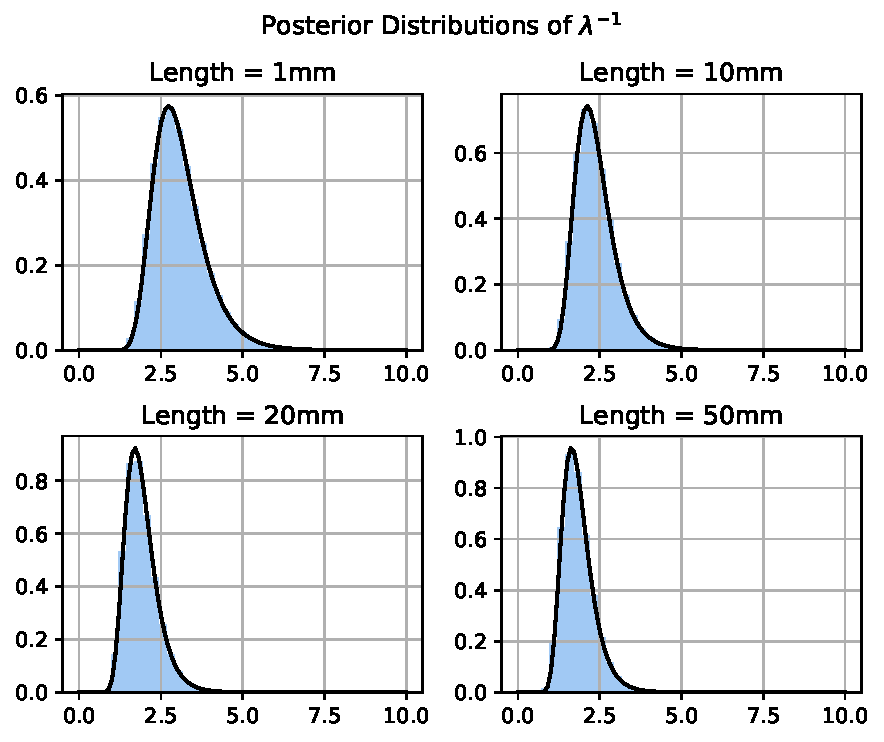
\includegraphics{p2_posterior_lambda_inverse.pdf}
          \caption{Histograms and probability density for samples drawn from the
            posteriors for $\lambda^{-1}$.}
          \label{fig:p2_posterior_lambda_inverse}
        \end{figure}

        Unlike the MLE, the posterior mean is not invariant under
        reparameterization:
        \[
          \mathbb{E}\left[\lambda^{-1} \mid Y\right] = \frac{b^\prime}{a^\prime - 1}
          \gneq  \frac{b^\prime}{a^\prime} = \frac{1}{\mathbb{E}\left[\lambda \mid Y\right]}.
        \]

        See
        \href{https://nbviewer.jupyter.org/github/ppham27/stat570/blob/master/hw4/failure\_stresses.ipynb}{\texttt{failure\_stresses.ipynb}} for code to reproduce plots.
      \end{description}
    \end{enumerate}
  \item In this question we will consider inference when the sampling model is
    multivariate hypergeometric. Suppose a population contains objects of $K$
    different types, with $X_1,\ldots,X_K$ being the number of each type,
    $\sum_{k=1}^K X_k = N$. A simple random sample of size $n$ is taken and the
    number of each type, $Y_1,\ldots,Y_K$, is recorded (so that
    $\sum_{k=1}^K y_k = n$).

    An obvious model for $Y_1,\ldots,Y_K$, is the multivariate hypergeometric
    distribution:
    \begin{equation}
      \mathbb{P}\left(Y_1 = y_1,\ldots,Y_K=y_K \mid x_1,\ldots,x_K\right) =
      \frac{\prod_{k=1}^K{x_k \choose y_k}}{{N \choose n}},
      \label{eqn:p3_hypergeometric}
    \end{equation}
    with means and variances:
    \begin{align}
      \mathbb{E}\left[Y_k \mid x_k\right]
      &= n\frac{x_k}{N} \label{eqn:p3_mean}\\
      \operatorname{Var}\left(Y_k \mid x_k\right)
      &= n\frac{x_k}{N}\left(1 - \frac{x_k}{N}\right)\frac{N-n}{N-1}.
        \label{eqn:p3_variance}
    \end{align}

    Suppose we take a sample from a population of $K$ distinct objects, and
    record $y_1,\ldots,y_K$, but the numbers $X_1,\ldots,X_K$ are unknown (but
    $N$ is known).
    \begin{enumerate}
    \item Using Equation \ref{eqn:p3_mean}, write down an estimator for $X_k$,
      $k = 1,\ldots,K$. We will refer to this a method of moments
      estimator. Using Equation \ref{eqn:p3_variance}, give a form for the
      variance of this estimator, along with the estimator of this variance.

      \begin{description}
      \item[Solution:] A simple estimator for $X_k$ can be obtained from
        Equation \ref{eqn:p3_mean} by substituting
        $\mathbb{E}\left[Y_k \mid x_k\right]$ with the observed $y_k$:
        \begin{equation}
          y_k = n\frac{\hat{x}_k}{N} \implies \hat{x}_k = \frac{N}{n}y_k.
          \label{eqn:p3_xk_method_of_moments}
        \end{equation}

        If we treat $\hat{x}_k$ like a random variable, then the variance of our
        estimator is
        \begin{align}
          \operatorname{Var}\left(\hat{x}_k\right)
          &= \operatorname{Var}\left(\frac{N}{n}Y_k\right)
            = \left(\frac{N}{n}\right)^2
            \operatorname{Var}\left(Y_k\right)\nonumber\\
          &= \left(\frac{N}{n}\right)^2\left(
            n\frac{x_k}{N}\left(1 - \frac{x_k}{N}\right)\frac{N-n}{N-1}
            \right) \nonumber\\
          &= x_k\left(\frac{N}{n}\right)
            \left(1 - \frac{x_k}{N}\right)\frac{N-n}{N-1}
            \label{eqn:p3_xk_method_of_moments_variance}
        \end{align}

        Since we don't know $x_k$, we substitute $x_k$ with $\hat{x}_k$ to get
        the estimated variance:
        \begin{align}
          \hat{\operatorname{Var}}\left(\hat{x}_k\right)
          &= \hat{x}_k\left(\frac{N}{n}\right)
            \left(1 - \frac{\hat{x}_k}{N}\right)\frac{N-n}{N-1} \nonumber\\
          &= y_k\left(\frac{N}{n}\right)^2
            \left(1 - \frac{y_k}{n}\right)\frac{N-n}{N-1} \nonumber\\
          &= \left(N - n\right)\frac{y_k}{n}\left(1 - \frac{y_k}{n}\right)
            \left(\frac{N^2}{n\left(N-1\right)}\right)
            \label{eqn:p3_xk_method_of_moments_variance_factored}
        \end{align}
      \end{description}
    \item We now consider a Bayesian approach to inference. Consider a
      multinomial distribution for counts $X_1,\ldots,X_K$,
      \begin{equation}
        \mathbb{P}\left(
          X_1 = x_1,\ldots,X_K = x_K \mid p_1,\ldots,p_K
        \right)
        = \frac{N!}{\prod_{k=1}^Kx_k!}\prod_{k=1}^K p_k^{x_k},
        \label{eqn:p3_multionomial}
      \end{equation}
      with $p_k > 0$ and $\sum_{k=1}^Kp_k = 1$. Show that the Dirichlet:
      \begin{equation}
        \pi\left(p_1,\ldots,p_K\right) = \frac{\Gamma\left(
            \alpha_+
          \right)}{\prod_{k=1}^K\Gamma\left(\alpha_k\right)}
        \prod_{k=1}^Kp_k^{\alpha_k-1},
        \label{eqn:p3_dirichlet}
      \end{equation}
      where $\alpha_k > 0$, $k = 1,\ldots,K$ and
      $\alpha_+ = \sum_{k=1}^K\alpha_k$ is the conjugate distribution to the
      multinomial sampling model.

      \begin{description}
      \item[Solution:] We use the definition of conjugate distributions and show
        that
        $\left(p_1,\ldots,p_K\right) \mid \left(X_1 = x_1,\ldots,X_K =
          x_k\right)$ is of the same distribution family as
        $\left(p_1,\ldots,p_K\right)$.

        We have that
        \begin{align}
          p\left(p_1,\ldots,p_K \mid x_1,\ldots,x_k\right)
          &\propto \mathbb{P}\left(
            x_1,\ldots,x_K \mid p_1,\ldots,p_K
            \right)\pi\left(p_1,\ldots,p_K\right) \nonumber\\
          &\propto \prod_{k=1}^K p_k^{x_k + \alpha_k - 1},
            \label{eqn:p3_posterior_propto}
        \end{align}
        which we recognize as the form of the Dirichlet family.

        Thus, we have that
        \begin{equation}
          p\left(p_1,\ldots,p_K \mid x_1,\ldots,x_k\right)
          =
          \frac{\Gamma\left(\alpha_+ + N\right)}{\prod_{k=1}^K\Gamma\left(\alpha_k + x_k\right)}
          \prod_{k=1}^K p_k^{\alpha_k + x_k  - 1},
          \label{eqn:p3_posterior}          
        \end{equation}
        so the Dirichlet distribution is the conjugate distribution to the
        multinomial sampling model.
      \end{description}
    \item The compound multinomial distribution,
      $\operatorname{CMult}\left(N,\alpha\right)$, is defined as
      \begin{equation}
        \mathbb{P}\left(
          X_1 = x_1,\ldots,X_K = x_K
        \right) =
        \frac{N!\Gamma\left(\alpha_+\right)}{\Gamma\left(N + \alpha_+\right)}
        \prod_{k=1}^K\frac{\Gamma\left(x_k + \alpha_k\right)}{x_k!\Gamma\left(\alpha_k\right)}
        \label{eqn:p3_compound_multinomial}
      \end{equation}
      where $\alpha = \left(\alpha_1,\ldots,\alpha_K\right)$. Show that the
      prior predictive distribution, obtained as the marginal distribution when
      the likelihood is Equation \ref{eqn:p3_multionomial} and the prior is
      Equation \ref{eqn:p3_dirichlet}, is of the compound multinomial
      form with parameters that you should identify.

      \begin{description}
      \item[Solution:] Let $\mathbf{p} = \left(p_1,\ldots,p_K\right)$. We simply
        integrate:
        \begin{align*}
          \mathbb{P}\left(
          X_1 = x_1,\ldots,X_K = x_K
          \right)
          &=
            \int \mathbb{P}\left(
            x_1,\ldots,x_K \mid p_1,\ldots,p_K
            \right) \pi\left(p_1,\ldots,p_K\right)\,\mathrm{d}\mathbf{p} \\
          &= 
            \frac{N!}{\prod_{k=1}^Kx_k!}
            \frac{\Gamma\left(
            \alpha_+
            \right)}{\prod_{k=1}^K\Gamma\left(\alpha_k\right)}
            \int
            \prod_{k=1}^K p_k^{x_k + \alpha_k - 1}
            \,\mathrm{d}\mathbf{p} \\
          &= \frac{N!\Gamma\left(\alpha_+\right)}{\prod_{k=1}^Kx_k!\Gamma\left(\alpha_k\right)}\left(
            \frac{\prod_{k=1}^K\Gamma\left(x_k + \alpha_k\right)}{\Gamma\left(N + \alpha_+\right)}
            \right) \\
          &= \frac{N!\Gamma\left(\alpha_+\right)}{\Gamma\left(N + \alpha_+\right)}
            \prod_{k=1}^K\frac{\Gamma\left(x_k + \alpha_k\right)}{x_k!\Gamma\left(\alpha_k\right)},
        \end{align*}
        where we have used that the Dirichlet probability density function must
        integrate to $1$ to compute the integral.
      \end{description}
    \item Find the mean $\mathbb{E}\left[X_k\right]$ and variance
      $\operatorname{Var}\left(X_k\right)$, $k = 1,\ldots,K$, of a compound
      multinomial distribution.

      \begin{description}
      \item[Solution:] We can use the law of total expectation for the mean:
        \begin{equation}
          \mathbb{E}\left[
            X_k
          \right] =
          \mathbb{E}_\pi\left[
          \mathbb{E}\left[
            X_k \mid p_k
          \right]
        \right]
        =
        \mathbb{E}_\pi\left[Np_k
        \right]
        = N\frac{\alpha_k}{\alpha_+},
        \label{eqn:p3_cmult_expectation}
      \end{equation}
      where we have taken advantage of the known means of the multinomial and
      Dirichlet distributions.

      For the variance we can use the law of total variance:
      \begin{align}
        \operatorname{Var}\left(X_k\right)
        &= \mathbb{E}_\pi\left[\operatorname{Var}\left(X_k \mid p_k\right)\right]
          + \operatorname{Var}\left(
          \mathbb{E}\left[
          X_k \mid p_k
          \right]
          \right) \nonumber\\
        &= \mathbb{E}_\pi\left[Np_k\left(1-p_k\right)\right]
          + \operatorname{Var}\left(Np_k\right)
          \nonumber\\
        &= N\left(\mathbb{E}_\pi\left[p_k\right] - \mathbb{E}_\pi\left[p_k^2\right]
          \right) + 
          N^2\operatorname{Var}\left(p_k\right) \nonumber\\
        &= N\left(\frac{\alpha_k}{\alpha_+}
          - \frac{\alpha_k\left(\alpha_+ - \alpha_k\right)}
          {\alpha_+^2\left(\alpha_+ + 1\right)} -
          \left(\frac{\alpha_k}{\alpha_+}\right)^2
          \right)
          + N^2\frac{\alpha_k\left(\alpha_+ - \alpha_k\right)}
          {\alpha_+^2\left(\alpha_+ + 1\right)} \nonumber\\
        &= N\frac{\alpha_k}{\alpha_+}\left(
          1 - \frac{1 + \alpha_k}{1 + \alpha_+}
          \right) +
          N\frac{\alpha_k}{\alpha_+}\left(N
          \frac{\alpha_+ - \alpha_k}{\alpha_+\left(\alpha_+ + 1\right)}
          \right) \nonumber\\
        &= N\frac{\alpha_k}{\alpha_+}
          \left(
          \frac{\alpha_+\left(\alpha_+ - \alpha_k\right)}{\alpha_+\left(1 + \alpha_+\right)} + 
          \frac{N\left(\alpha_+ - \alpha_k\right)}{\alpha_+\left(1 + \alpha_+\right)}
          \right) \nonumber \\
        &= N\frac{\alpha_k}{\alpha_+}
          \left(
          \frac{\left(\alpha_+ - \alpha_k\right)\left(N + \alpha_+\right)}{\alpha_+\left(1 + \alpha_+\right)}\right) \nonumber\\
        &= N\frac{\alpha_k}{\alpha_+}
          \left(
          1 - \frac{\alpha_k}{\alpha_+}
          \right)
          \left(
          \frac{N + \alpha_+}{1 + \alpha_+}
          \right).
        \label{eqn:p3_cmult_variance}
      \end{align}
    \end{description}
  \item Let $W_k = X_k - y_k$ represent the unobserved counts, $k= 1,\ldots,K$.
    Show that the posterior distribution
    $\mathbb{P}\left(W_1,\ldots,W_K|y_1,\ldots,y_K\right)$ is compound multinomial
    $\operatorname{CMult}\left(N-n,\alpha+y\right)$, where $y= (y_1,\ldots,y_K)$.

    \begin{description}
    \item[Solution:] Given $y$, $W = \left(W_1,\ldots,W_K\right)$ is just a
      reparameterization of $X = \left(X_1,\ldots,X_k\right)$. However, the
      domain is different since $W_k \geq 0$, so we need a normalization
      constant.

      Using Equation \ref{eqn:p3_compound_multinomial} as our prior and Equation
      \ref{eqn:p3_hypergeometric} as our likelihood, we can compute the posterior
      \begin{align}
        \mathbb{P}
        &\left(
          W_1 = w_1,\ldots,W_K = w_K
          \mid y_1,\ldots,y_K
          \right) \nonumber\\
        &\propto \mathbb{P}\left(
          y_1,\ldots, y_K
          \mid X
          \right)          
        \mathbb{P}\left(
          X_1 = w_1 + y_1,
          \ldots,
          X_K = w_K + y_K
          \right) \nonumber\\
        &\propto
          \left(\frac{\prod_{k=1}^K{w_k + y_k \choose y_k}}{{N \choose n}}\right)
          \left(\frac{N!\Gamma\left(\alpha_+\right)}{\Gamma\left(N + \alpha_+\right)}
          \prod_{k=1}^K\frac{\Gamma\left(w_k + y_k + \alpha_k\right)}{\left(w_k + y_k\right)!\Gamma\left(\alpha_k\right)}\right) \nonumber\\
        &\propto
          \frac{\left(N - n\right)!n!\Gamma\left(\alpha_+\right)}{\Gamma\left(N + \alpha_+\right)}
          \prod_{k=1}^K\frac{\Gamma\left(w_k + y_k + \alpha_k\right)}{w_k!y_k!\Gamma\left(\alpha_k\right)} \nonumber\\
        & \propto \prod_{k=1}^K\frac{\Gamma\left(w_k + y_k + \alpha_k\right)}{w_k!},
          \label{eqn:p3_posterior_w_propto}
      \end{align}nn
      which we recognize as the from the compound multionomial
      distribution. Since Equation \ref{eqn:p3_posterior_w_propto} must sum to 1
      to be a proper probability distribution over the support of the prior
      $\sum_{k=1}^K W_k = N - n$, where $W_k$ are nonnegative integers, we get that      
      \begin{align}
        \mathbb{P}
        &\left(
          W_1 = w_1,\ldots,W_K = w_K
          \mid y_1,\ldots,y_K
          \right) \nonumber\\
        &= \frac{\left(N - n\right)!\Gamma\left(n + \alpha_+\right)}{\Gamma\left(\left(N - n\right) + \left(n + \alpha_+\right)\right)}
          \prod_{k=1}^K\frac{\Gamma\left(w_k + \left(y_k + \alpha_k\right)\right)}{w_k!\Gamma\left(y_k + \alpha_k\right)},
          \label{eqn:p3_posterior_w}  
      \end{align}
      which is the $\operatorname{CMult}\left(N - n, y + \alpha\right)$
      distribution.      
    \end{description}
  \item Write down the posterior mean and posterior variance of $X_k$,
    $k= 1,\ldots,K$.  Comment on the case when $\alpha_k = 0$, $k = 1,\ldots,K$.
    \begin{description}
    \item[Solution:] Using the results from Equation \ref{eqn:p3_posterior_w},
      \ref{eqn:p3_cmult_expectation}, and \ref{eqn:p3_cmult_variance}, we have
      \begin{align}
        \mathbb{E}\left[
        X_k \mid y_1,\ldots,y_K
        \right]
        &= \mathbb{E}\left[
          W_k \mid y_1,\ldots,y_K
          \right] + y_k \nonumber\\
        &= y_k + \left(N - n\right)\frac{y_k + \alpha_k}{n + \alpha_+}.
          \label{eqn:p3_posterior_x_expectation} \\
        \operatorname{Var}\left(X_k \mid y_1,\ldots,y_K \right)
        &= \operatorname{Var}\left(W_k \mid y_1,\ldots,y_K \right) \label{eqn:p3_posterior_x_variance}
        \\
        &= \left(N - n\right)\frac{y_k + \alpha_k}{n + \alpha_+}
          \left(1 - \frac{y_k + \alpha_k}{n + \alpha_+}\right)
          \left(\frac{N + \alpha_+}{1 + n + \alpha_+}\right). 
          \nonumber  
      \end{align}

      When $\alpha = \mathbf{0}$, the expectation and variance are similar to
      those of the multinomial distribution with $p_k = y_k/n$, but the variance
      has the additional $\frac{N}{1 + n}$ factor. These are similar to the
      method of the moments estimators in Equations
      \ref{eqn:p3_xk_method_of_moments} and
      \ref{eqn:p3_xk_method_of_moments_variance_factored}. The mean estimate is
      same as posterior mean, and the variance has a
      $\frac{N^2}{n\left(N - 1\right)}$ has is quite close to $\frac{N}{1 + n}$,
      especially for large values of $N$ and $n$.
    \end{description}
  \item A certain infectious disease can be caused by one of three different
    pathogens, A, B, or C. Over a 1 year period population surveillance is
    carried out, and 750 individuals are observed to be infected. A random
    sample of 60 cases is selected for labtesting, i.e., to determine the
    pathogen responsible.  Of these 60 selected cases,the numbers who were
    infected by pathogens A, B, C, were 42, 18, 0, respectively. We wish to
    estimate the numbers of the total population of cases that were infected by
    each of the pathogens.

    \begin{enumerate}
    \item Calculate the method of moments estimators and the associated standard
      errors.

      \begin{description}
      \item[Solution:] Let $X_1$, $X_2$, and $X_3$ correspond to the total
        population with pathogens A, B, and C, respectively. Let $Y_1$, $Y_2$,
        and $Y_3$ be the corresponding samples.

        We substitute $N = 750$, $n = 60$, $y_1 = 42$, $y_2 = 18$, and
        $y_3 = 0$ into Equations \ref{eqn:p3_xk_method_of_moments} and
        \ref{eqn:p3_xk_method_of_moments_variance}.

        For the estimated means, we have
        \begin{align}
          \hat{x}_1
          &= 750\frac{42}{60} = 525 \nonumber\\
          \hat{x}_2
          &= 750\frac{18}{60} = 225 \nonumber\\
          \hat{x}_3
          &= 750\frac{0}{60} = 0.
            \label{eqn:p3_method_of_moment_means}
        \end{align}

        For estimated standard errors, we have
        \begin{align}
          \sqrt{\hat{\operatorname{Var}}\left(\hat{x}_1\right)}
          &\approx 42.587 \nonumber\\
          \sqrt{\hat{\operatorname{Var}}\left(\hat{x}_2\right)}
          &\approx 42.587 \nonumber\\
          \sqrt{\hat{\operatorname{Var}}\left(\hat{x}_3\right)}
          &= 0. \label{eqn:p3_method_of_moment_standard_errors}
        \end{align}
                
      \end{description}
    \item Calculate the Bayesian posterior mean and posterior standard
      deviation, with prior specification, $\alpha_k= 1$, $k= 1,\ldots,K$. Which
      estimates are the most reasonable?
      \begin{description}
      \item[Solution:] Here, we substitute into Equations
        \ref{eqn:p3_posterior_x_expectation} and
        \ref{eqn:p3_posterior_x_variance}.

        We have that
        \begin{align}
          \mathbb{E}\left[X_1 \mid y\right]
          &= 42 + \left(690\right)\frac{42 + 1}{60 + 3} = 42 + \frac{9890}{21}
            \approx 512.952 \nonumber\\
          \mathbb{E}\left[X_2 \mid y\right]
          &= 18 + \left(690\right)\frac{18 + 1}{60 + 3} = 18 + \frac{4370}{21}
            \approx 226.095 \nonumber\\
          \mathbb{E}\left[X_3 \mid y\right]
          &= 0 + \left(690\right)\frac{1}{63} = \frac{230}{21} \approx 10.952,
            \label{eqn:p3_posterior_mean_examples}
        \end{align}
        and
        \begin{align}
          \sqrt{\operatorname{Var}\left[X_1 \mid y\right]}
          &\approx 41.941 \nonumber\\
          \sqrt{\operatorname{Var}\left[X_2 \mid y\right]}
          &\approx 41.352 \nonumber\\
          \sqrt{\operatorname{Var}\left[X_3 \mid y\right]}
          &\approx 11.261.
            \label{eqn:p3_posterior_variance_examples}
        \end{align}

        The estimates in Equations \ref{eqn:p3_posterior_mean_examples} and
        \ref{eqn:p3_posterior_variance_examples} are similar to those in
        Equations \ref{eqn:p3_method_of_moment_means} and
        \ref{eqn:p3_method_of_moment_standard_errors} for $X_1$ and $X_2$ but
        are pulled slightly closer together since the prior specifies that the
        pathogens occur in about equal proportions.

        The estimate for $X_3$ is much different, however. In Equations
        \ref{eqn:p3_method_of_moment_means} and
        \ref{eqn:p3_method_of_moment_standard_errors}, the estimate and standard
        error is $0$ because there were no observations. If we know that at
        least one person carries pathogen C, this estimate is deeply
        disturbing. It could simply be that no one in our sample carried the
        pathogen, so the Bayesian estimates are most reasonable.
      \end{description}
    \end{enumerate}
  \end{enumerate}
  \end{enumerate}
\end{document}
